\documentclass{svproc}
\usepackage{graphicx} 
\usepackage{amsmath}
\usepackage{biblatex}
\usepackage{soul} %for highlighting
\usepackage{xcolor} %for highlighting
\addbibresource{lit.bib}

\title{Exploring the effectiveness of Small-Scale Vision and Language Models for Vision and Language Navigation Tasks in Continuous Environments}
\author{Wesley Chiu, Abdulrahman Altahhan}
\institute{University of Leeds, School of Computing, ODL MSc in AI, UK. \\ \texttt{\{od22wc, a.altahhan\}@leeds.ac.uk}}
\date{January 2025}
\begin{document}
\maketitle

\begin{abstract}
    Vision-and-Language Navigation (VLN) is a rapidly evolving field of research that aims to enable an embodied agent to follow textual instructions given in natural language to navigate through an unseen environment to a goal position. Existing approaches to this ask all into two main categories: "specialist" models that have been constructed and trained specifically to solve this task, and zero-shot or few-shot models that aim to leverage the implicit knowledge within Large Language Models (LLMs) and Vision Language Models  (VLMs). Prior work in the latter approach have used the most powerful models (70B+ parameters). This work aims to evaluate the suitability of using a lighter-weight variant of an existing open-sourced model (Qwen2-VL) as the primary VLM, which would allow it to be run "on-device" rather than being connected to a broader network. The experiments in a simulated environment demonstrates that the current ability of the lighter-weight model is not yet fit for purpose, failing to reach the success rates seen in approaches that use the full-sized variants.
    
    \keywords{Vision-and-Language Navigation, Vision Language Model, Large Language Model, Prompt Engineering, Prompting}
\end{abstract}

\section{Introduction}
    Vision and Language Navigation (VLN) is a rapidly evolving field of research, which tasks an embodied agent to follow a set of textual instructions given in natural language to navigate a previously unseen 3D indoor environment. Whilst initial research leveraged models such as RNNs and CNNs to process visual and natural language data, the introduction of Transformer-based models \cite{attenion_is_all_you_need} has accelerated capabilities in Natural Language Processing (NLP) and Computer Vision (CV) - both key components in the VLN task. The rapid development of Large Language Models (LLMs) and Vision-Language Models (VLMs) has further intensified the volume and pace of research in VLN, with each advance in LLM and VLM competency directly benefiting the VLN task.
    The traditional VLN task, as proposed by Andersen, et al. in 2017 \cite{8578485}, has the agent navigate between pre-defined nodes in the environment (sometimes referred to as a navigation graph), which essentially reduces the VLN task to a vision-based graph-search problem; models trained in this manner have difficulty translating to performance in the real-world \cite{pmlr-v155-anderson21a}. To help combat this gap, the VLN Continuous Environment (VLN-CE) task was introduced, and has no such predefined navigation points, requiring agents to take low-level actions to reach a navigable point in the environment. This introduces new challenges for the models to overcome, such as avoiding getting stuck on obstacles and dealing with distances \cite{krantz2020navgraphvisionandlanguagenavigationcontinuous}.
    \newline \par
    Approaches to the VLN task (whether graph-based VLN or VLN-CE) that leverage existing LLMs and VLMs typically fall into two broad categories: 'generalist' models or 'specialist' models.
    \par
    Generalist models \cite{long2023_discussnav, chen2024mapgptmapguidedpromptingadaptive, zhou2023navgptexplicitreasoningvisionandlanguage} use 'off-the-shelf' models such as OpenAI's ChatGPT \cite{openai2024gpt4technicalreport} and aim to leverage the implicit knowledge, NLP ability, and strong reasoning skills within LLMs and VLMs \cite{51647, LMs_as_knowledge_bases} to navigate the environment. These approaches rely on specific prompting to generate historical trajectories, make navigation decisions, and to monitor progress.
    \par
    Specialist models \cite{hong2021_vlnbert, navgpt2, chen2021_HAMT, HE2024110511_MemoryAdaptiveVLN} are built from the ground-up, typically with specialist sub-models, to tackle the VLN task. These approaches exhibit stronger performance in VLN tasks compared to the generalist approach, but are less unable to take advantage of more competent LLMs or VLMs as they are released in the same 'plug-and-play' manner of generalist models.
    \newline
    Both approaches typically leverage larger, complex language and vision models, requiring powerful hardware with high amounts of memory to run during inferencing. The development of Low Rank Adaptation (LoRA) finetuning \cite{LoRA} combined with model quantization \colorbox{yellow}{citation required} allows for a LLM or VLM to be trained and run on hardware with more limited memory. This is particularly relevant to the VLN task, as lighter-weight models can be run more readily on smaller robots with more limited hardware, broadening the application of these models.
    \newline
    This work explores the effectiveness of using a small, finetuned, quantized open-sourced model as the primary VLM to tackle the VLN-CE task and examines its performance against other generalist approaches. 
    
\section{Literature Review}
    \textbf{Vision and Language Navigation (VLN)}  The ability for an embodied agent to navigate a previously unseen environment purely by natural language instruction is a field of research that has seen increasing interest since the task was formally introduced by Andersen et al. in 2017 \cite{8578485}. The VLN task requires that an embodied agent be able to navigate an unstructured and previously unseen environment by following navigation instructions provided in natural language. Early research focused on the use of Recurrent Neural Networks (RNNs) \cite{8578485, 8954045, 8953608}; however, with the introduction of the Transformer archicture \cite{attenion_is_all_you_need} and the subsequent development of the Large Language Model (LLM) \cite{radford2018improving, touvron2023llamaopenefficientfoundation}, recent research has focused on leveraging the NLP capabilities of LLMs; these approaches can be broadly categorised into two different approaches: a text-based approach and an integrated approach.
    \par The text-based approach seeks to address the challenge of multi-modality by translating visual features from the agent's observations into textual space. LangNav \cite{pan2024langnavlanguageperceptualrepresentation} and NavGPT \cite{zhou2023navgptexplicitreasoningvisionandlanguage}, for example, used image captioning models such as BLIP \cite{li2022blipbootstrappinglanguageimagepretraining, li2023blip2bootstrappinglanguageimagepretraining} and DETR \cite{zhu2021deformabledetrdeformabletransformers} to caption images and identify objects in those images; this textual information was then passed to GPT4 for decision making and other navigation tasks; OpenNav \cite{open-nav} takes a similar approach with open-sourced models. Variations on this approach include DiscussNav \cite{long2023_discussnav}, which uses a similar mechanism to enable discussions between its multiple domain experts, as well as NavCOT \cite{lin2024navcotboostingllmbasedvisionandlanguage}, which asks the LLM to predict information about observations from future states.
    
    more recent research has expanded to investigate different model pre-training strategies \cite{9156554, Guhur_2021_ICCV} as well as Zero or Few-shot VLN agents. 
    \\ \\
    \textbf{Large Language Models and Vision Models in VLN}  ... (talk about LangNav and others) (use of GPT) (generalised vs specialist models) (Open-Nav uses Qwen2-72B?)
    \\ \\
    \textbf{Vision Language Models}
    \\ \\
    \textbf{Challenges in Continuous Environments} ... (talk about Sim2Real challenges) (speak about work that used node-based navigation)
    \newline
    However, these models typically rely on translating visual data into purely textual information, which risks a loss of information in the process \cite{pan2024langnavlanguageperceptualrepresentation}; as a result, these models typically underperform against specialist models. The strength of these models lie in the fact that no pre-training is required, and as LLMs and VLMs continue to improve, this increase in competency can directly translate into improved VLN performance without the need for pre-training or adaptation of a complex model structure.

\section{Methodology}
    The approach taken in this work, as illustrated in \colorbox{yellow}{Figure 1}, comprises of using a single VLM as the primary component of the model to help the model understand where it located in the environment, track its historical trajectory, and to make decisions on its next action. A small component of this architecture leverages an LLM to break down the natural language instructions into discrete "Navigation Checkpoints", which is in line with prior work \cite{ chen2024mapgptmapguidedpromptingadaptive, pan2024langnavlanguageperceptualrepresentation, zhou2023navgptexplicitreasoningvisionandlanguage}.
    
\subsection{Problem Formulation}
    The VLN-CE task asks an embodied agent to autonomously navigate from a specified starting point to a goal location in an unseen environment by following a path described by natural language instructions. That is, given a natural language navigation instruction $\mathcal{I}$ and a starting state $S_0$, at each step $t$ the agent must determine its current location in the environment and its current progress to take an action $a_t$ that will lead it closer to the goal state $S_G$. The agent determines through observations $O_t$ obtained from its sensors. In this work, $O_t$ is comprised of colour images $I$ from $N$ different views, each set at a different angle, from the egocentric perspective of the agent. Additionally, the agent is also able to observe the environment through an egocentric panoramic image $I_{p,t}$. That is, the observations at each step is represented by $O_t = \{o_{p,t}, o_{0, t}, ..., o_{N,t}\}$. At each step, the agent must choose to take an action which corresponds to an image direction (excluding $o_{p,t}$), i.e. $a_t \in \{o_{0,t}, ..., o_{N,t}\}$, unless a specific direction is determined to result in a collision with the environment, in which case that particular direction is removed from the action set.

    The agent is deemed to have successfully reached $S_G$ if the final state of the agent $S_T$, where $T$ is the total number of steps taken, is within 1.0 metres of $S_G$.

\subsection{Framework and Prompts}
    Unlike prior work that used separate Vision and Language models \cite{zhou2023navgptexplicitreasoningvisionandlanguage, 51647} which require pre-training to combine the different models, this work proposes the use of a singular VLM to manage both the image and textual inputs.
    \par The VLM is used for inference for three different purposes: to track Navigation History, Decide the Next Checkpoint to work toward, and to Decide the Next Step. Only one task, creating Inferred Navigation Checkpoints, is not given to the VLM, and is instead given to the LLM. 
    \\ \\
    \textbf{Inferred Navigation Checkpoints}  The navigation instructions provided by the RxR dataset is given in natural language, and can include discourse markers that may not be relevant to the navigation itself (e.g. \texttt{"Okay, now ..."}) and may be confusing or difficult to track progress against. To address this, this work follows prior work \cite{open-nav,navgpt2} an LLM is used to convert $\mathcal{I}$ into a list of Navigation Checkpoints, which is easier for the model to track progress against. That is, for each $\mathcal{I}$, a series of $M$ Navigation Checkpoints $C = \{C_0, ..., C_M\}$ are created such that by progressing from $c_0$ (the starting point of the instruction) to $c_M$ will result in a successful trajectory (i.e. $S_T \leq S_G\pm  1.0 \text{ metres}$).
    \\ \\
    \textbf{Navigation History}  A key component to the success of VLN agents is that at the time of deciding the optimal $a_{t+1}$ the agent has the capability to retain in its context a history of its navigational trajectory \cite{chen2021_HAMT, HE2024110511_MemoryAdaptiveVLN}.
    \par In this work, at each step, the VLM is prompted to generate $h_t$, which is a summary of the reasoning given for selecting $a_t$ and the agent's current location based on $o_{p,t}$. The VLM is provided with $C$, $o_{p,t}$, ${a_t}$ and the reasoning associated with its selection as the best action, as well as the Navigation History $H_{t-1} = \{h_{t'}, ..., h_{t-1}\}$, where $t' = \text{max}(t-20, 0)$. Once generated, $h_t$ is appended to the Navigation History, such that $H_t = \{h_{t'+1}, ..., h_t\}$. The Navigation History is limited to only the past 20 steps to manage VRAM limitations in the hardware; however, this also prevents actions taken much earlier, which are unlikely to be relevant to the current action, from entering the VLM's context window, thereby removing some noise from the data \cite{HE2024110511_MemoryAdaptiveVLN}.
    \\ \\
    \textbf{Deciding Next Checkpoint}  Each Navigation Checkpoint $c_m$ acts as an medium-term goal for the agent to navigate toward, which is particularly important in trajectories where $S_G$ is not visible from $S_0$. At each step, the VLM is provided with $C$, $O_t$, and $H_t$ and is then prompted to state the list of all the Navigaton Checkpoints the agent has already achieved ($c_0$ to $c_{m-1}$), the Navigation Checkpoint the agent should now be working toward $c_m$, and the instructions associated with $c_m$.
    \\ \\
    \textbf{Deciding Next Step}  The VLN-CE task requires the agent to decide at each step which of the low-level actions would be most likely to lead to $c_m$. At each step, the VLM is provided with $O_t$ and the reasoning associated with $c_m$ described in the "Deciding Next Checkpoint" section above. The VLM is then prompted to repeat the instructions for $c_m$ and to select the $o_n$ that is most aligned with that Navigation Checkpoint. During prompting, the list of available actions for that step ($A_t$) is modified to remove the action \texttt{"Forward"} if the simulation detects a collision if that step were to be taken; this is an emulation of a Laser Distance Scanner providing collision information to the agent and provides some environmental feedback to the agent.

\subsection{Finetuning Data Generation for Continuous Environment}
    Each natural language navigation instruction provided by the RxR dataset is paired with a set of waypoints that describes the path that the original annotator used to create the instructions. This path can be referred to as the "gold label" trajectory that the agent should follow to reach the goal in as direct an approach as possible. As the instructions were created using the Matterport3D simulator \cite{Matterport3D}, a navigation-graph based simulator, the provided waypoints do not describe a path that is relevant to the VLN CE task.
    \\ \\
    \textbf{Gold Label Trajectory}  The original trajectories from the RxR \textit{train} split were used to determine a new "gold label" trajectory for use in the continuous environment (CE-Trajectory). The agent was placed at the starting state $S_0$, and at each step $t$, all potential actions $\{a_{t,0}', ..., a_{t,N}'\}$ were assessed by determining the state that each action would result in $\{S_{t+1,0}', ..., S_{t+1,N}'\}$. The next best action was determined in a greedy manner by the state $s_{t+1}$ that was closest to the next waypoint in the original trajectory; this was repeated until $S_T \leq S_G \pm 1.0 \text{ metres}$.
    \par
    Some of the RxR annotations and waypoints describe trajectories and actions that the agent specified in this work cannot take, or would require a material deviation from the original trajectory to achieve. For example, some of these instructions may include: \texttt{"Hop over the coffee table"}, \texttt{"Hop over the table"}, or navigating to an outdoor staircase. To avoid these trajectories, any trajectories where $T > 50$ were rejected, resulting in 3,304 eligible CE-Trajectories.
    \\ \\
    \textbf{Generating Training Prompts}  The training data required for finetuning the VLM requires that the training data include the prompts for the \texttt{user} and \texttt{assistant} roles. These prompts were generated by recreating the experience described in the "gold label" trajectories and capturing the prompts used in the Navigation History and Progress Monitor modules. A slightly adjusted version of the Action Decider module, the Action Rationalizer, was created to \textit{rationalise} the decision behind the provided action $a_t$ at each step. The same process was used to create the calibration dataset for use in quantization.

\section{Experiment}
\subsection{Datasets and Environment Simulation}
    \textbf{Dataset}  The Matterport3D \cite{Matterport3D} dataset is a well known and commonly used dataset in VLN research. It comprises of 194,400 colour and depth (RGB-D) images to create panoramas at 10,800 different (internal) locations from 90 different residential buildings. These panoromas allows a Matterport user to view the environment in full in 360\textdegree, and also allows users to "teleport" from one panoramic "node" to another. These panoramic nodes form the "navigation-graph" used in traditional or discrete VLN models.
    The Room-across-Room (RxR) dataset \cite{mattersim, rxr} was used for the natural language instructions, which comprises of over 126,000 natural language instructions (annotations) across three different languages to describe traversal through 16,500 different paths in the Matterport3D dataset. For this work, only the en-US guide annotations were considered, which comprises of 13,992 annotations across 13,992 unique paths. Finally, the annotations are separated into the following splits: \textit{train}, \textit{seen val}, and \textit{unseen val}. In order to align with prior work, the \textit{train} split was used for generating finetuning data, whilst the \textit{unseen val} split was used to test the model.
    \newline \newline
    \textbf{Environment}  Habitat-Sim \cite{habitat19iccv, szot2021habitat, puig2023habitat3} was used as the simulated environment, which converts the navigation graph-based Matterport3D dataset into continous environments. The environment was also set to allow sliding, which allows the agent to slide along an obstacle rather than being stuck against it. The agent in the simulator was given a colour sensor, through which colour images could be captured for the agent to observe the envrionment in. The agent was able to observe its environment in 6 different directions: Forward (0\textdegree, straight ahead), Forward-left (45\textdegree to its left, as measured from the forward direction), Left (90\textdegree to its left), Forward-right (45\textdegree to its right), Right (90\textdegree to its right), and Behind (180\textdegree from its forward direction); each observation has a 90\textdegree horizontal and vertical field of view (FOV). The agent is able to take an action that corresponds to each of these observations, where "Forward" would result in a forward step of 1.0 metres, whilst all other actions would result in the agent turning to face that direction (e.g. "Forward-left" would result in turning 45\textdegree to the left). The agent was also provided a colour sensor to create a panoramic colour observation, with an effective horizontal FOV of 360\textdegree and a vertical FOV of 90\textdegree.
    
\subsection{Implementation Details}
    This work used a finetuned and quantized open-sourced VLM as the primary model to navigate an environment. All finetuning, quantization and inferencing of the model was run on a desktop computer with an AMD Ryzen 7 7800x3D CPU, 32GB of RAM, and an NVIDIA RTX4090 with 24GB of VRAM.

    Qwen2-VL-7B-Instruct \cite{Qwen-VL, Qwen2VL} was chosen as the base model for the VLM due to its strong performance relative to other open-sourced models \cite{vlm_leaderboard} of similar parameter size.
    The model was finetuned using Low Rank Adaptation (LoRA) \cite{LoRA}, and quantized using Activation-aware Weight (AWQ) optimisation \cite{MLSYS2024_42a452cb}. Both model finetuning and qunatization were conducted through LLaMa-Factory \cite{zheng2024llamafactory}.

    OpenAI's ChatGPT 4 \cite{openai2024gpt4technicalreport} was chosen as the LLM, which was used solely to convert the natural language navigation instructions from the RxR dataset into a structured list of Navigation Checkpoints.

\subsection{Experiment Results}
    \textbf{Results} were ...

\section{Conclusion and Future Work}

\section{Reference Code bit}
    This is how you reference stuff: \ref{fig:fig2}


    \begin{figure}
        \centering
        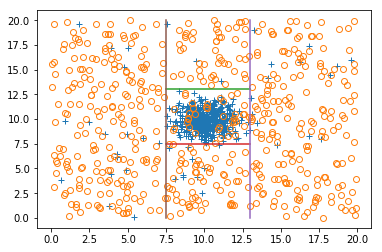
\includegraphics[scale=.75]{figures/DecisionBoundary.png}
        \caption{Caption}
        \label{fig:fig2}
    \end{figure}

    
    \begin{figure}
        \centering
        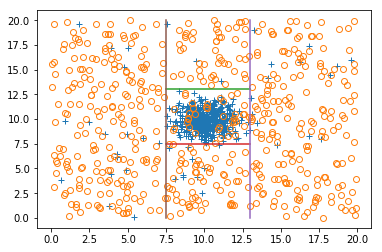
\includegraphics[scale=.75]{figures/DecisionBoundary.png}
        \caption{Caption}
        \label{fig:my_label}
    \end{figure}


    
    In Fig. \ref{fig:my_label} that $\alpha = n^2$. In eq. (\ref{eq:sum_i}) we have shown that the $ 1+2+3+4 = 4\times 5 /2=10$.
    \begin{align*}
        \sum_{i=1}^{n} y &= 10 \\
        M &= \beta ^2 \\
        \boldsymbol{B}^\top &= \boldsymbol{\Lambda}^2 \\
    \end{align*}
    
    \begin{align}
        \label{eq:sum_i}
        \sum_{i=1}^n i &= \frac{(n+1)n}{2} \\  
        \nonumber
        \beta ^2 &= \alpha_i^n
    \end{align}

\section{Experiment Results}
    \subsection{Experiment 1}
        \subsubsection{Exp}
    Note that the figure and the tables might be laid out on another page. Do not worry about that, and do not attempt to change it. Leave this to Latex.
    
    
    \begin{table}
        \caption{This is a table}
        \begin{center}
            \begin{tabular}{rlc}
                \hline
                \multicolumn{1}{l}{Year}&\multicolumn{1}{l}{World}&\multicolumn{1}{l}{Duration}\\
                \hline
                8000 B.C.  &     5,000,000 &  10\\
                  50 A.D.  &   200,000,000 &  20\\
                1650 A.D.  &   500,000,000 &  30\\
                \hline
            \end{tabular}
        \end{center}
    \end{table}

\section{Conclusion and Future Work}
We have conducted a study on ...

\printbibliography 
\end{document}
